\section{Proposed Architecture}
\label{proposed_architecture_section}

The overall architecture is shown in Figure \ref{proposed_architecture}. By interacting with the environment, the agent accumulates state transition experiences, which is used by ILASP to learn a hypothesis.
The agent also record surrounding information it has seen as background knowledge, which will be used to make a plan together with the hypothesis that ILASP learns. 
Each steps are described in details below. 

\begin{figure}[!htb]
\centering
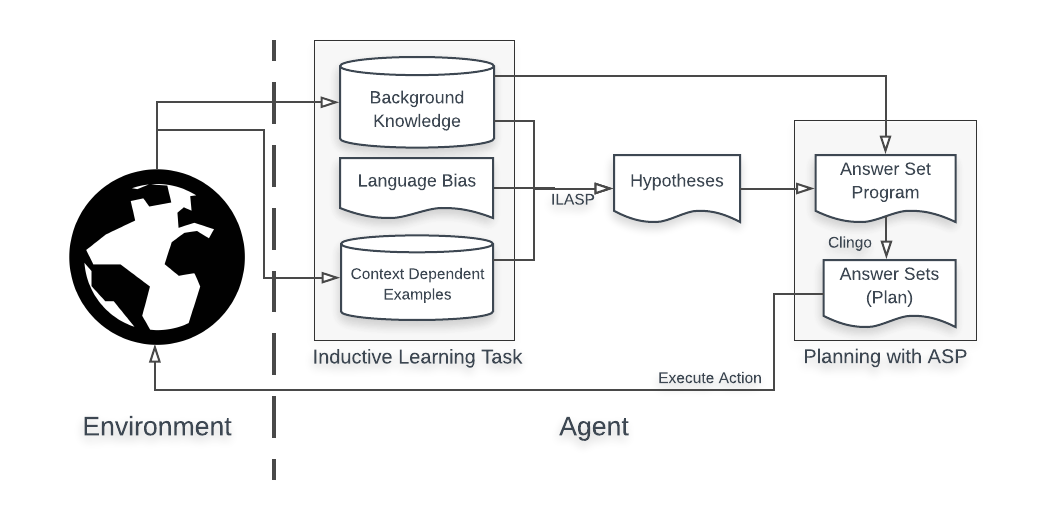
\includegraphics[width=1.0\textwidth]{./figures/architecture}
% 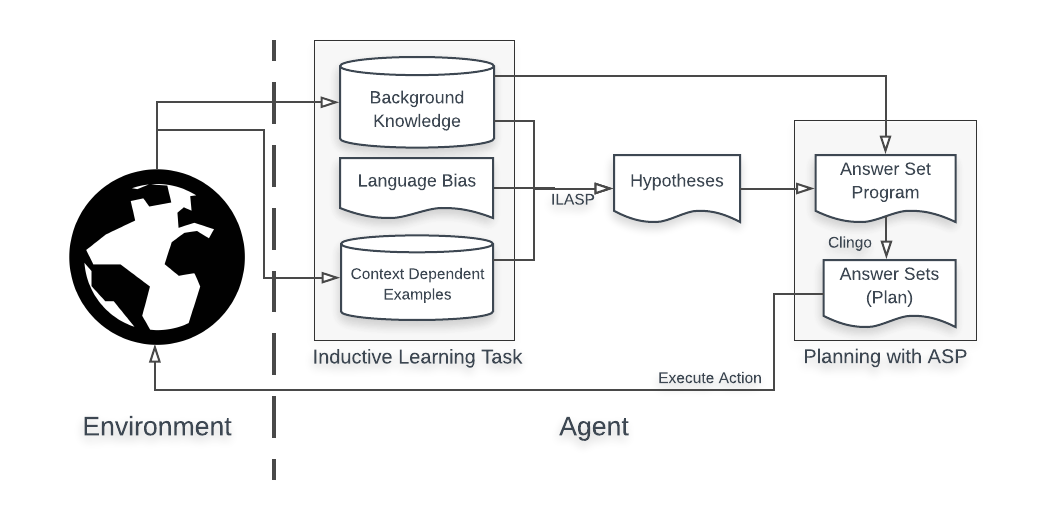
\includegraphics[width=10cm, height=9cm]{./figures/architecture}
\caption{Proposed reinforcement learning architecture. ILASP learns to generate a model and updates based on the interaction with the environment, which is used to hypothesis. }
\label{proposed_architecture}
\end{figure}

\subsection{Experience Accumulation}
\label{experience_accumulation}

The first step is to accumulate experience by interacting with the environment. The agent explores the environment randomly until it reaches the goal once. 
Every time the agent takes an action during the exploration phase, these experiences need to be recorded in two ways: state transition experience and environment experience.

\subsubsection{State transition experience}
State transition experiences will be used as E in ILASP, especially positive examples for ILASP in ASP syntax, which is of the form

\#pos({state\_after((X2,Y2))}, {all other state\_after that did not happen}, {state\_before((X1,Y1)). action(A). surrounding information}).

where ,  
\begin{itemize}
    \item inclusions contain one state\_after((X2,Y2)), which represents the position of the agent in x and y axis after an action is taken 
    \item exclusions contain all other state\_after((X,Y)) that did not occur
    \item context example include state\_before((X1,Y1)), which represents the position of the agent in x and y axis before an action is taken,
    action(A) is the action the agent has taken, and surrounding information, such as walls, if any. 
\end{itemize}


At the first stage, the input of real experience needs to be converted in ASP form, which can be used to execute the inductive learning in ILASP. The input used in ILASP is state transitions, 
rewards and an action of the agent, which can be directly converted using a simple mapping table or an action language (such as BC\textsuperscript{+} as used in \cite{Ferreira2017}). 
The following ASP input is what is sent to ILASP. \\

There is no negative example as XXXX. 

\begin{examp} \normalfont (Positive examples). 

Suppose an agent takes an action "up" to move from (1,3) to (1,4) cell. All other alternative states that the agent could have ended up by taking different actions 
(down, right, left, and not move) are in the exclusions. Finally surrounding walls information are in the context.

\#pos(\{state\_after((1,3))\}, \\
    \{state\_after((2,4)),state\_after((1,5)),state\_after((0,4)),state\_after((1,4))\}, \\
    \{state\_before((1,4)). action(up). wall((1, 5)). wall((0, 4)). \})



This example will be used to learn how to move up as one of the agent's hypotheses.

Another example is 

\#pos({state\_after((1,3))}, {state\_after((2,3)),state\_after((1,4)),state\_after((0,3)),state\_after((1,2))}, {state\_before((1,3)). action(up). wall((2, 3)). wall((0, 3)). wall((1, 2)). }).

where the agent tried to move up, from (1,3) to (1,2), but ended up in the same cell at (1,3). This is because there is a wall at (1,2), and the agent learns in order to move an above cell,
there must not be a wall in the above cell. 

\end{examp}
\label{state_transition_example}

% TODO do I need this??
agent\_at\_before((X,Y), T).

agent\_at\_after((X,Y), T).

reward(R, T).

action(A, T).

\subsubsection{Environment experience}

While the agent explores in the environment, it also remembers all the surrounding information as background knowledge, 
which will be used to generate a sequence of actions plan using H. In a simple maze, these could be all wall position that the agent has seen so far, which can be 

wall((1, 5)). which represents the location of the wall. 

Another example could be a location of a teleportation if the agent sees it. 

These environment experiences are part of context examples in the positive examples. 

Together with the positive examples (E) as described above. 

\subsection{Inductive Learning}
\label{induction}

Once the agent hits the goal once, ILASP gets triggered and try to learn a hypothesis using the positive examples the agent accumulated so far. 

generate hypothesis H,

In addition to the positive examples, the following definitions are supplied

cell((0..7, 0..6)). \\
\#modeb(1, link(var(cell), var(cell)), (positive)). \\
% (X+1,Y) is right next to (X,Y)
adjacent(right, (X+1,Y),(X,Y))   :- cell((X,Y)), cell((X+1,Y)). \\
adjacent(left,(X,Y),  (X+1,Y)) :- cell((X,Y)), cell((X+1,Y)). \\
% (X,Y+1) is above next to (X,Y)
adjacent(down, (X,Y+1),(X,Y))   :- cell((X,Y)), cell((X,Y+1)). \\
adjacent(up,   (X,Y),  (X,Y+1)) :- cell((X,Y)), cell((X,Y+1)). \\

\#modeh(state\_after(var(cell))). \\
\#modeb(1, adjacent(const(action), var(cell), var(cell))). \\
\#modeb(1, state\_before(var(cell)), (positive)). \\
\#modeb(1, action(const(action)),(positive)). \\
\#modeb(1, wall(var(cell))). \\

Without these in the form of mode bias, the search space for ILASp will be empty. 
Positive excludes the possibility of negation as a failure in order to reduce the search space.

\#max\_penalty(100).

By default it is XX, 

\#constant(action, right).
\#constant(action, left).
\#constant(action, down).
\#constant(action, up).
\#constant(action, non).

The actions in the body have to be constant

Together with the above defition as well as accumulated positive examples, ILASP is able to learn an hypothesis. The quality of H depends on the experiences for the agent. 
For example, In the early phase of learning, the agent does not have many examples, and learns an hypothesis that may not be insightfull. 
For example, if the agent has only one positive example, 

XXX

The learnt hypothesis is XXX

This hypothesis, for example, does not explain how to move "down". In order to learn how to move "down", it needs an positive example of moving up. 

later on H improving as we collect more examples as well as background knowledge.

state\_after(V0) :- adjacent(right, V0, V1), state\_before(V1), action(right), not wall(V0).
state\_after(V0) :- adjacent(left, V0, V1), state\_before(V1), action(left), not wall(V0).
state\_after(V0) :- adjacent(down, V0, V1), state\_before(V1), action(down), not wall(V0).
state\_after(V0) :- adjacent(up, V0, V1), state\_before(V1), action(up), not wall(V0).

These learnt H will be used to generate a plan in the abduction phase. 

After executing the plan, the agent will have more positive examples, which will be used to improve the quality of H. 

\subsection{Generate a plan}
\label{Generate a plan}

Generate a plan using abduction

If the hypotheses were not accurate, clingo might not generate all the actions leading to the goals. 

\subsection{Plan execution}
\label{Plan execution}

the plan generated by clingo is a set of states and actions. 

states are of the form state\_at((X,Y),T), where X and Y represent x-axi and y-axi in a maze respectively, T represents a time that the agent is at 
this particular X,Y cell. 

action(A,T) tells which action the agent should take at each time. By following the actions, the agent should collect both predicted state that the 
agent will end up, and the observed state that the agent actually end up. If there is a difference between these two, either B or H do not correctly represent
the model of the true environment, so needs to be improved. 

When the agent encounters a new environment (e.g a new wall), this new information will be added to its background, which will be used to improved the hypothesis 
next time ILASP gets executed. 

For example, 

state\_at((1,1),1) action(right,1)
state\_at((2,1),2) action(right,2)
state\_at((3,1),3) action(right,3)
state\_at((4,1),4) action(right,4)
state\_at((5,1),5)


At the start of the learning, H is usually not correct or too general, using this H will generate lots of answer sets that are not useful for the planning. 
These examples will be collected and included as exclusions of a new positive example. 

For example, 
XXX


To avoid the agent from being stuck in a sub-optimal plan, the agent deliberately discards the plan and takes an random action with a probability of 
epsilon (which is less than 1) TODO define this mathematically. 
When the agent deviates from the planning, it often discovers new information, which will be added to B.
Exploration is necessary to make sure that the agent might discovers a shorter path than the current plan, which will be demonstrated in the experiment. 

Define them here

Our algorithm works by 

It buids the model of the environment by improving two internal concepts: hypothesis H and background knowledge B. 
% First, an agent explores an environment by taking random actions until it reaches the goal. 


In the further research, we could experiment with a more sophisticated exploration strategy, such as XXX and YYY. 


This is formally defined in Algorithm. 

\begin{algorithm}
\caption{ILASP(RL)}\label{euclid}
\begin{algorithmic}[1]
\Procedure{ILASP(RL) (B and E)}{}

\While {True}

    \State $\textit{H (inductive solutions)} \gets \text{run ILASP(T)}$
    \State $\textit{plan(actions, states) answer sets} \gets \text{AS(B, H)}$
    \While {actions in P}
        \State $\textit{observed state} \gets \text{run clingo(T)}$
        \If {$ \textit{observed state} \neq \textit{predicted state} $}
            \State $\textit{H} \gets \text{run ILASP(T)}$
            \EndIf
        % \If {$ \textit{observed state not equal \textit{predicted state $} 
        % \EndIf
    \EndWhile
    % \If {$ new \ background \ encountered $}
    %     % \State $\textit{H} \gets \text{run ILASP(T)}$
    % \EndIf
    % \For{i from 0 to N} 
    %     \If {$ A[i]\ is \ in \ T$}
    %         \State \Return $FALSE$
    %     \Else 
    %         \State Add A[i] to T   
    %     \EndIf
    % \EndFor
% \State \Return $TRUE$
\EndWhile

\EndProcedure
\caption{XXXX }
\end{algorithmic}
\end{algorithm}

\subsection{Model Generation and Update using ILASP}
\label{model_generation_and_update}
Once the input of the real experience is converted into ASP syntax, the agent should learn the following definition of the model of the environment using ILASP. \\

valid\_move(C, T):- link(C, T).
\\
link(C2, T):- agent\_at(C1, T), adjacent(C0, C2), not obstacle(C0, C2).\\
%state\_transition(C1, C2, T2):-
%  agent\_at\_before(C1, T1),
%  agent\_at\_after(C2, T2).\\
agent\_at(C, T):- agent\_at\_after(C, T) \\

The background knowledge is empty, and there are only positive examples in learning this task. Each example contains a different transition history of the agent. 
Inclusions are valid moves and exclusions are invalid moves. 
Learning valid\_move is the same as learning the rule of the games (the model of the environment), and it is updated as the agent explores in the environment.

In addition to the rules of the game, learning the following concepts will be crucial for transfer learning, as these concepts will be applicable to any types of game environment.  \\

adjacent(C1, C2):- cell(C1), cell(C2). \\
%obstacle(C1, C2):- enemy(C1, C2). \\
obstacle(C1, C2):- wall(C1, C2). \\
wall(C1, C2):- agent\_at\_before(C1, T1), agent\_at\_after(C1, T2) \\
enemy(C1, C2):- agent\_at\_before(C1, T1), agent\_at\_after(C2, T2), reward(R), -100 $\geq$ R \\

where it is assumed that the reward of -100 means losing the game or losing the agent's life. 
Once the agent has learned the concept of the game, it knows how to avoid an obstacle in an adjacent cell in a new environment. 
Figure \ref{grid_world} illustrates this transfer capability.

\begin{itemize}

\item States: XXX
\item Actions: The agent can move up, down, right or left
\item Rewards: XXX
\item Transitions: XXX

\end{itemize}
